\documentclass[dutch]{ucll-slides}
\usepackage{pxfonts}
\usepackage{tikz}
\usepackage{calc}
\usepackage{ucll-code}
\usepackage{siunitx}


\usetikzlibrary{calc,shadows,tikzmark,shapes.multipart,math}

\coursename{Scripttalen}
\title{Lambda's}

\newcommand{\nonterminal}[1]{{\color{red} \ensuremath{\langle}#1\ensuremath{\rangle}}}

\newenvironment{matchexamples}{
  \begin{center}
  \newcommand{\sep}{\hspace{5mm}}
  \newcommand{\match}[1]{\sep{\color{green!50!black} "##1"}}
  \newcommand{\mismatch}[1]{\sep{\color{red} "##1"}}
}{\end{center}}




\begin{document}

\maketitle

\begin{frame}
  \frametitle{Vragen}
  \code[language=java,width=.85\linewidth,font=\small]{main.java}
  \codeunderlinex{args}
  \begin{itemize}
    \item Wat is het nut van de \texttt{main} parameters?
    \item Wat is het nut van een shell?
    \item Hoe kunnen meerdere processen met elkaar praten?
    \item Hoe interageert men met bestanden?
  \end{itemize}
\end{frame}


%%% Local Variables:
%%% mode: latex
%%% TeX-master: "io"
%%% End:


\begin{frame}
  \frametitle{Werkvoorbeeld}
  \code[language=python]{person.py}
\end{frame}

\section{Selecties}

\frame{\tableofcontents[currentsection]}

\begin{frame}
  \frametitle{Volwassenen Selecteren}
  \begin{quote}
    Gegeven een lijst \texttt{Person}s, selecteer
    alle meerderjaardigen ($18 \leq \mathrm{age}$).
  \end{quote}
  \code[language=python]{selectAdults.py}
\end{frame}

\begin{frame}
  \frametitle{Honderdjarigen Selecteren}
  \begin{quote}
    Gegeven een lijst \texttt{Person}s, selecteer
    alle \texttt{Person}s die ouder zijn dan 100 ($100 \leq \mathrm{age}$).
  \end{quote}
  \code[language=python]{selectCentennials.py}
\end{frame}

\begin{frame}
  \frametitle{Veralgemening: \texttt{selectOlderThan}}
  \begin{itemize}
    \item \texttt{select\_adults} selecteert $\mathrm{age} \geq 18$
    \item \texttt{select\_centennials} selecteert $\mathrm{age} \geq 100$
    \item Twee verschillende functies met quasi zelfde implementatie
    \item Samenvoegen in \'e\'en veralgemeende functie
  \end{itemize}
  \code[language=python]{selectOlderThan.py}
\end{frame}

\begin{frame}
  \frametitle{Jonge Volwassenen Selecteren}
  \begin{quote}
    Gegeven een lijst \texttt{Person}s, selecteer
    alle jonge volwassenen ($18 \leq \mathrm{age} \leq 25$).
  \end{quote}
  \vskip5mm
  \begin{overprint}
    \onslide<1>
    \code[language=python3,font=\small,width=.9\linewidth]{selectYoungAdults.py}

    \onslide<2>
    \code[language=python3,font=\small,width=.9\linewidth]{selectYoungAdults2.py}
  \end{overprint}
  \vskip5mm
  \begin{overprint}
    \onslide<1>
    \begin{center}
      Zeer gelijkaardig aan \texttt{select\_adults}\dots \\
      Kunnen we misschien \texttt{select\_older\_than} herbruiken?
    \end{center}

    \onslide<2>
    \begin{center}
      Klungelig
    \end{center}
  \end{overprint}
\end{frame}

\begin{frame}
  \frametitle{Veralgemening: \texttt{selectWithAgeBetween}}
  \begin{itemize}
    \item Wat als we $18 \leq \mathrm{age} \leq 65$ willen selecteren?
    \item We veralgemenen weeral
    \item \texttt{select\_older\_than} ontving minimale leeftijd
    \item We voegen maximale leeftijd parameter toe
  \end{itemize}
  \vskip5mm
  \code[language=python3,font=\small,width=.95\linewidth]{selectWithAgeBetween.py}
\end{frame}

\begin{frame}
  \frametitle{Andere Selecties}
  \structure{Andere Mogelijke Selecties}
  \begin{itemize}
    \item Selecteer alle Jannen
    \item Selecteer zij die meer dan \SI{80}{\kilogram} wegen
    \item Selecteer zij die groter zijn dan \SI{2}{\meter}
    \item Selecteer zij die een BMI hoger dan 30 hebben
  \end{itemize}
  \vskip5mm
  \structure{Implementatie}
  \begin{itemize}
    \item Allemaal selectie-opdrachten
    \item Hoe dit veralgemenen naar \'e\'en functie?
  \end{itemize}
\end{frame}

\begin{frame}
  \frametitle{Poging Tot Veralgemening}
  \code[language=python3,font=\tiny]{selectPersons.py}
\end{frame}

\begin{frame}
  \frametitle{Evaluatie \texttt{selectPersons}}
  \begin{itemize}
    \item \emph{Verschrikkelijk} onhandig
    \item Veel typwerk $\rightarrow$ veel kans op bugs
    \item Moet herhaald worden voor elke klasse
    \item Kan nog altijd niet willekeurige selecties aan
          \begin{itemize}
            \item Selecteer namen die beginnen op F
            \item Selecteer zij die jonger zijn dan 18 \emph{of} lichter zijn dan \SI{50}{\kilogram}
            \item Selecteer zij die \emph{niet} Jan heten
          \end{itemize}
    \item Is absoluut geen aanvaardbare oplossing
  \end{itemize}
\end{frame}

\begin{frame}
  \frametitle{Wat Als\dots}
  \begin{itemize}
    \item Zou handig zijn indien Python een {\tt filter} lus aanbood
  \end{itemize}
  \code[language=python3,font=\small,width=.9\linewidth,extra keywords={filter}]{filter-loop.py}
  \begin{itemize}
    \item Werkt met willekeurige selectie-condities
    \item Werkt op willekeurige objecten (niet enkel \texttt{Person}s)
  \end{itemize}
\end{frame}


%%% Local Variables:
%%% mode: latex
%%% TeX-master: "lambdas"
%%% End:

\section{Projecties}

\frame{\tableofcontents[currentsection]}

\begin{frame}
  \frametitle{Opvragen Namen}
  \begin{quote}
    Gegeven een lijst \texttt{Person}s, wat zijn hun namen?
  \end{quote}
  \code[language=python]{getNames.py}
\end{frame}

\begin{frame}
  \frametitle{Opvragen Leeftijden}
  \begin{quote}
    Gegeven een lijst \texttt{Person}s, wat zijn hun leeftijden?
  \end{quote}
  \code[language=python]{getAges.py}
\end{frame}

\begin{frame}
  \frametitle{Veralgemening: \texttt{getFields}}
  \code[language=python3,font=\small,width=.9\linewidth]{getFields.py}
  \begin{itemize}
    \item \texttt{getattr} kan gebruikt worden om waarde veld op te vragen
    \item \texttt{get\_fields} werkt op alle types objecten
    \item \texttt{get\_fields} werkt voor alle veldnamen
  \end{itemize}
\end{frame}

\begin{frame}
  \frametitle{Opvragen BMIs}
  \begin{quote}
    Gegeven een lijst \texttt{Person}s, wat zijn hun BMI's?
  \end{quote}
  \code[language=python3,font=\small,width=.95\linewidth]{getBMIs.py}
  \begin{itemize}
    \item \texttt{get\_fields} werkt \emph{enkel} op velden
    \item Bewerkingen nodig $\rightarrow$ weer terugvallen op manuele lus
  \end{itemize}
\end{frame}

\begin{frame}
  \frametitle{Wat Als\dots}
  \begin{itemize}
    \item Zou handig zijn indien Python een {\tt map} lus aanbood
  \end{itemize}
  \code[language=python3,font=\small,width=.9\linewidth,extra keywords={map}]{map-loop.py}
  \begin{itemize}
    \item Willekeurige bewerkingen op willekeurige objecten
  \end{itemize}
\end{frame}

%%% Local Variables:
%%% mode: latex
%%% TeX-master: "lambdas"
%%% End:

\section{Andere ``Lussen''}

\frame{\tableofcontents[currentsection]}

\begin{frame}
  \frametitle{Tellen Van Volwassenen}
  \begin{quote}
    Tel het aantal volwassen personen.
  \end{quote}
  \vskip5mm
  \begin{overprint}
    \onslide<1>
    \code[language=python]{countAdults.py}

    \onslide<2>
    \code[language=python, extra keywords={count}]{count-loop.py}
  \end{overprint}
\end{frame}

\begin{frame}
  \frametitle{Is Iedereen Volwassen?}
  \begin{quote}
    Zijn alle \texttt{Person}s in de lijst volwassen?
  \end{quote}
  \vskip5mm
  \begin{overprint}
    \onslide<1>
    \code[language=python]{allAdults.py}

    \onslide<2>
    \code[language=python, extra keywords={all}]{all-loop.py}
  \end{overprint}
\end{frame}

\begin{frame}
  \frametitle{Is Er Een Volwassene?}
  \begin{quote}
    Is er minstens \'e\'en \texttt{Person} uit de lijst volwassen?
  \end{quote}
  \vskip5mm
  \begin{overprint}
    \onslide<1>
    \code[language=python]{anyAdults.py}

    \onslide<2>
    \code[language=python, extra keywords={any}]{any-loop.py}
  \end{overprint}
\end{frame}

\section{First Class Functions}

\frame{\tableofcontents[currentsection]}

\begin{frame}
  \frametitle{Potenti\"ele Nieuwe Lussen}
  \structure{In Voorgaande Voorbeelden}
  \begin{itemize}
    \item \texttt{filter}
    \item \texttt{map}
    \item \texttt{count}
    \item \texttt{all}
    \item \texttt{any}
  \end{itemize}
  \begin{center} \itshape
    Kunnen we  deze lussen zelf implementeren?
  \end{center}
  \visible<2->{
    \begin{center}
      Ja!
    \end{center}
  }
\end{frame}

\begin{frame}
  \frametitle{\texttt{filter} Als Functie: Stapsgewijze Opbouw}
  \begin{overprint}
    \onslide<1>
    \code[language=python3,font=\small]{selectAdults2.py}
    \codeunderline{selectAdults start}{selectAdults end}

    \onslide<2>
    \code[language=python3,font=\small]{selectAdults3.py}
    \codeunderline[name center=selectAdults2 center 1]{selectAdults2 start1}{selectAdults2 end1}
    \codeoverline[name center=selectAdults2 center 2]{selectAdults2 start2}{selectAdults2 end2}
    \tikz[remember picture,overlay] \draw[thick,red,-latex] let \p1=(selectAdults2 center 2), \p2=(selectAdults2 center 1) in (\p1) -- ++(0,0.1) -- ++(2.5,0) |- ($ (\p2) + (0,-0.4) $) -- (\p2);

    \onslide<3>
    \code[language=python3,font=\small]{selectAdults4.py}
    \codeunderline[name center=selectAdults3 center 1]{selectAdults3 start1}{selectAdults3 end1}
    \codeoverline[name center=selectAdults3 center 1b,stroke/.style={thick,blue}]{selectAdults3 start1}{selectAdults3 end1}
    \codeoverline[name center=selectAdults3 center 2]{selectAdults3 start2}{selectAdults3 end2}
    \codeoverline[name center=selectAdults3 center 3,stroke/.style={thick,blue}]{selectAdults3 start3}{selectAdults3 end3}
    \tikz[remember picture,overlay] \draw[thick,red,-latex] let \p1=(selectAdults3 center 2), \p2=(selectAdults3 center 1) in (\p1) -- ++(0,0.5) |- ($ (\p2) + (0,-0.4) $) -- (\p2);
    \tikz[remember picture,overlay] \draw[thick,blue,-latex] let \p1=(selectAdults3 center 3), \p2=(selectAdults3 center 1b) in (\p1) -- ++(0,0.1) -- ++(3,0) |- ($ (\p2) + (0,0.3) $) -- (\p2);
  \end{overprint}
\end{frame}

\begin{frame}
  \frametitle{\texttt{map} Als Functie}
  \begin{overprint}
    \onslide<1>
    \code[language=python3,font=\small]{getAges2.py}
    \codeoverline{getAges2 start}{getAges2 end}

    \onslide<2>
    \code[language=python3,font=\small]{getAges3.py}
    \codeunderline[name center=getAges3 center 1]{getAges3 start1}{getAges3 end1}
    \codeoverline[name center=getAges3 center 2]{getAges3 start2}{getAges3 end2}
    \tikz[remember picture,overlay] \draw[thick,red,-latex] let \p1=(getAges3 center 2), \p2=(getAges3 center 1) in (\p1) -- ++(0,1) |- ($ (\p2) + (0,-0.4) $) -- (\p2);

    \onslide<3>
    \code[language=python3,font=\small]{getAges4.py}
    \codeunderline[name center=getAges4 center 1]{getAges4 start1}{getAges4 end1}
    \codeoverline[name center=getAges4 center 1b,stroke/.style={thick,blue}]{getAges4 start1}{getAges4 end1}
    \codeoverline[name center=getAges4 center 2]{getAges4 start2}{getAges4 end2}
    \codeoverline[name center=getAges4 center 3,stroke/.style={thick,blue}]{getAges4 start3}{getAges4 end3}
    \tikz[remember picture,overlay] \draw[thick,red,-latex] let \p1=(getAges4 center 2), \p2=(getAges4 center 1) in (\p1) |- ($ (\p2) + (0,-0.4) $) -- (\p2);
    \tikz[remember picture,overlay] \draw[thick,blue,-latex] let \p1=(getAges4 center 3), \p2=(getAges4 center 1b) in (\p1) -- ++(0,0.1) -- ++(5,0) |- ($ (\p2) + (0,0.3) $) -- (\p2);
  \end{overprint}
\end{frame}

\begin{frame}
  \frametitle{First Class Functions}
  \begin{itemize}
    \item In Python zijn functies ``first class citizens''
          \begin{itemize}
            \item Mogelijk om functies mee te geven als argument
            \item Mogelijk om functies te returnen
            \item Mogelijk om functies in variabelen te bewaren
          \end{itemize}
    \item Een functie is een object
    \item Operatie \texttt{()} dient om functie op te roepen
  \end{itemize}
  \code[language=python3,font=\small]{first-class-function.py}
\end{frame}

\begin{frame}
  \frametitle{Bestaande Functies}
  \code[language=python]{map.py}
\end{frame}

\begin{frame}
  \frametitle{Bestaande Functies}
  \code[language=python]{filter.py}
\end{frame}

\begin{frame}
  \frametitle{Bestaande Functies}
  \code[language=python]{any.py}
\end{frame}

\begin{frame}
  \frametitle{Bestaande Functies}
  \code[language=python]{all.py}
\end{frame}


%%% Local Variables:
%%% mode: latex
%%% TeX-master: "lambdas"
%%% End:

\section{Lambda's}

\frame{\tableofcontents[currentsection]}

\begin{frame}
  \frametitle{Opvragen Velden van \texttt{Person}-objecten}
  \begin{overprint}
    \onslide<1>
    \code[language=python]{map-names.py}
    \onslide<2>
    \code[language=python]{map-ages.py}
    \onslide<3>
    \code[language=python]{map-heights.py}
  \end{overprint}
  \vskip4mm
  \begin{center}
    \begin{tikzpicture}[scale=0.75,transform shape,
                        person/.style={draw,rectangle split,rectangle split parts=2,minimum width=4cm,drop shadow,fill=white},
                        value/.style={draw,minimum width=4cm,fill=white,drop shadow}]
      \pgfdeclarelayer{background}
      \pgfsetlayers{background,main}

      \node[person] (jan) at (0,0) {
        \textbf{Person}
        \nodepart{two}
        \begin{tabular}{r@{$\;=\;$}l}
          name & Jan \\
          age & 18 \\
          height & 186 \\
          weight & 92 \\
        \end{tabular}
      };
      \node[person,anchor=south west] (piet) at ($ (jan.south east) + (1,0) $)  {
        \textbf{Person}
        \nodepart{two}
        \begin{tabular}{r@{$\;=\;$}l}
          name & Piet \\
          age & 19 \\
          height & 173 \\
          weight & 69 \\
        \end{tabular}
      };
      \node[person,anchor=south west] (tom) at ($ (piet.south east) + (1,0) $)  {
        \textbf{Person}
        \nodepart{two}
        \begin{tabular}{r@{$\;=\;$}l}
          name & Tom \\
          age & 23 \\
          height & 182 \\
          weight & 75 \\
        \end{tabular}
      };

      \node[value,anchor=north] (jan value) at ($ (jan.south) + (0,-1) $) {%
        \only<1>{Jan}%
        \only<2>{18}%
        \only<3>{186}%
      };
      \node[value,anchor=north] (piet value) at ($ (piet.south) + (0,-1) $) {%
        \only<1>{Piet}%
        \only<2>{19}%
        \only<3>{173}%
      };
      \node[value,anchor=north] (tom value) at ($ (tom.south) + (0,-1) $) {%
        \only<1>{Tom}%
        \only<2>{23}%
        \only<3>{182}%
      };

      \draw[-latex] (jan.south) -- (jan value.north);
      \draw[-latex] (piet.south) -- (piet value.north);
      \draw[-latex] (tom.south) -- (tom value.north);

      \begin{pgfonlayer}{background}
        \path[fill=red!25] ($ (jan.north west) + (-0.2,0.2) $) rectangle ($ (tom.south east) + (0.2,-0.2) $);
        \path[fill=red!25] ($ (jan value.north west) + (-0.2,0.2) $) rectangle ($ (tom value.south east) + (0.2,-0.2) $);
      \end{pgfonlayer}
    \end{tikzpicture}
  \end{center}
\end{frame}

\begin{frame}
  \frametitle{Hulpfuncties}
  \begin{itemize}
    \item Opvragen naam: functie \texttt{get\_name}
    \item Opvragen leeftijd: functie \texttt{get\_age}
    \item Opvragen lengte: functie \texttt{get\_height}
    \item Opvragen gewicht: functie \texttt{get\_weight}
    \item Telkens nieuwe functie nodig per veld
    \item Veel typwerk (boilerplate code)
  \end{itemize}
\end{frame}

\begin{frame}
  \frametitle{Lambda's}
  \begin{itemize}
    \item Zulke kleine hulpfuncties vaak nodig
    \item Kortere notatie mogelijk
    \item ``Inline functie''
  \end{itemize}
  \vskip5mm
  \begin{overprint}
    \onslide<1-3>
    \code[language=python]{map-names-lambda.py}
    \only<2>{
      \codeunderlinex{getName p}
      \codeoverlinex{lambda p}
      \begin{tikzpicture}[remember picture,overlay]
        \draw[thick,red,latex-] (getName p) -- ++(0,-1) -| (lambda p);
      \end{tikzpicture}
    }
    \only<3>{
      \codeunderlinex{getName body}
      \codeoverlinex{lambda body}
      \begin{tikzpicture}[remember picture,overlay]
        \draw[thick,red,latex-] (getName body) -- ++(0,-1) -| (lambda body);
      \end{tikzpicture}
    }

    \onslide<4>
    \code[language=python]{map-ages-lambda.py}

    \onslide<5>
    \code[language=python]{map-heights-lambda.py}
  \end{overprint}
\end{frame}

\begin{frame}
  \frametitle{Lambda's}
  \begin{center}
    \ttfamily {\bfseries lambda} \nonterminal{args}:\ \nonterminal{body}
  \end{center}
  \begin{itemize}
    \item Body moet \'e\'en expressie zijn
    \item Impliciete \texttt{return}
    \item Stelt een anonieme functie voor
  \end{itemize}
\end{frame}

\begin{frame}
  \frametitle{Lambda's in Andere Talen}
  \begin{itemize}
    \item First class functions en lambda's niet Python-specifiek
          \begin{itemize}
            \item Java sinds versie 8
            \item C++ sinds C++11
            \item C$^\sharp$
            \item JavaScript
            \item dots
          \end{itemize}
    \item Hebben meerdere doeleinden
          \begin{itemize}
            \item Vervangen lussen
            \item Parallellisme
            \item Asynchrone operaties
          \end{itemize}
  \end{itemize}
\end{frame}

%%% Local Variables:
%%% mode: latex
%%% TeX-master: "lambdas"
%%% End:

\section{List Comprehensions}

\frame{\tableofcontents[currentsection]}

\begin{frame}
  \frametitle{List Comprehensions}
  \begin{itemize}
    \item {\tt map} en {\tt filter} worden vaak gebruikt
    \item Python biedt specifieke syntax
  \end{itemize}
  \vskip5mm
  \begin{overprint}
    \onslide<1>
    \code[language=python,font=\small,width=.98\linewidth]{list-comprehension.py}
    \onslide<2>
    \code[language=python,font=\small,width=.98\linewidth]{list-comprehension2.py}
  \end{overprint}
\end{frame}


%%% Local Variables:
%%% mode: latex
%%% TeX-master: "lambdas"
%%% End:


\end{document}


%%% Local Variables: 
%%% mode: latex
%%% TeX-master: t
%%% End: 
